\documentclass[landscape,paperheight=24in,fontscale=.45,paperwidth=36in,landscape,final]{baposter}

\usepackage{times}
\usepackage{calc}
\usepackage{amsmath}
\usepackage{amssymb}
\usepackage{relsize}
\usepackage{multirow}
\usepackage{bm}
\usepackage{tikz}
\usepackage{graphicx}
\usepackage{float}
\usepackage{multicol}
\usepackage{subfigure}
\usepackage{color}
\usepackage{pgfbaselayers}
\usepackage{subfigure}
\pgfdeclarelayer{background}
\pgfdeclarelayer{foreground}
\pgfsetlayers{background,main,foreground}

% \usepackage{helvet}
% %\usepackage{bookman}
% \usepackage{palatino}

\usepackage[T1]{fontenc}
\usepackage{ae}

% \newcommand{\captionfont}{\footnotesize}

\selectcolormodel{rgb}

\graphicspath{{images/}}

%%%%%%%%%%%%%%%%%%%%%%%%%%%%%%%%%%%%%%%%%%%%%%%%%%%%%%%%%%%%%%%%%%%%%%%%%%%%%%%%
% Multicol Settings
%%%%%%%%%%%%%%%%%%%%%%%%%%%%%%%%%%%%%%%%%%%%%%%%%%%%%%%%%%%%%%%%%%%%%%%%%%%%%%%%
\setlength{\columnsep}{0.7em}
\setlength{\columnseprule}{0mm}


%%%%%%%%%%%%%%%%%%%%%%%%%%%%%%%%%%%%%%%%%%%%%%%%%%%%%%%%%%%%%%%%%%%%%%%%%%%%%%%%
% Save space in lists. Use this after the opening of the list
%%%%%%%%%%%%%%%%%%%%%%%%%%%%%%%%%%%%%%%%%%%%%%%%%%%%%%%%%%%%%%%%%%%%%%%%%%%%%%%%
\newcommand{\compresslist}{%
\setlength{\itemsep}{1pt}%
\setlength{\parskip}{0pt}%
\setlength{\parsep}{0pt}%
}


\definecolor{silver}{cmyk}{0,0,0,0.3}
\definecolor{yellow}{cmyk}{0,0,0.9,0.0}
\definecolor{reddishyellow}{cmyk}{0,0.22,1.0,0.0}
\definecolor{black}{cmyk}{0,0,0.0,1.0}
\definecolor{darkYellow}{cmyk}{0,0,1.0,0.5}
\definecolor{darkSilver}{cmyk}{0,0,0,0.1}

\definecolor{lightyellow}{cmyk}{0,0,0.3,0.0}
\definecolor{lighteryellow}{cmyk}{0,0,0.1,0.0}
\definecolor{lighteryellow}{cmyk}{0,0,0.1,0.0}
\definecolor{lightestyellow}{cmyk}{0,0,0.05,0.0}

\definecolor{lightblues}{rgb}{.867, .918, .965}
\definecolor{mediumblues}{rgb}{.617, .789, .879}
\definecolor{darkblues}{rgb}{.191, .508, .738}

\definecolor{ColorBrew1}{rgb}{166, 97, 26}
\definecolor{ColorBrew2}{rgb}{223, 194, 125}
\definecolor{ColorBrew3}{rgb}{245, 245, 245}
\definecolor{ColorBrew4}{rgb}{128, 205, 193}
\definecolor{ColorBrew5}{rgb}{1, 133, 113}

\definecolor{textborder}{rgb}{0,0,156}
\definecolor{textheaderdark}{rgb}{0,0,156}
\definecolor{textheaderlight}{rgb}{0,0,156}

\definecolor{DukeBlue}{HTML}{001A57}
\definecolor{LBlue}{HTML}{336699}
\definecolor{Teal}{HTML}{BFBFBF}
%\definecolor{DukeBlue}{rgb}{0,0,.6}
%\definecolor{DukeBlue}{rgb}{0,0,.611764706}



%%%%%%%%%%%%%%%%%%%%%%%%%%%%%%%%%%%%%%%%%%%%%%%%%%%%%%%%%%%%%%%%%%%%%%%%%%%%%%
%%% Begin of Document
%%%%%%%%%%%%%%%%%%%%%%%%%%%%%%%%%%%%%%%%%%%%%%%%%%%%%%%%%%%%%%%%%%%%%%%%%%%%%%
\begin{document}

%%%%%%%%%%%%%%%%%%%%%%%%%%%%%%%%%%%%%%%%%%%%%%%%%%%%%%%%%%%%%%%%%%%%%%%%%%%%%%
%%% Here starts the poster
%%%---------------------------------------------------------------------------
%%% Format it to your taste with the options
%%%%%%%%%%%%%%%%%%%%%%%%%%%%%%%%%%%%%%%%%%%%%%%%%%%%%%%%%%%%%%%%%%%%%%%%%%%%%%
\typeout{Poster Starts}
\background{}

\begin{poster}{
  % Show grid to help with alignment
  grid=false,
  columns=4,
  % Column spacing
  colspacing=1em,
  % Color style
  bgColorOne=white, %specified the background color of the entire chart
  bgColorTwo=black, % not sure what this does
  borderColor=Teal,  % border color of boxes on poster
  headerColorOne=LBlue,  % color of header
  headerColorTwo=black,  % not sure what this does
  headerFontColor=white, % color of font
  boxColorOne=white,
  boxColorTwo=white,
  % Format of textbox
  textborder=rounded,
  % Format of text header
  eyecatcher=true,
  headerborder=open,
  headerheight=0.08\textheight,
  headershape=roundedright,
  headershade=plain,
  headerfont=\large\textsc, %Sans Serif
  boxshade=plain,
%  background=shade-tb,
  background=plain,
  linewidth=2pt
  }
{
Eye Catcher, empty if option eyecatcher=no
}
{
\textcolor{LBlue}{Making Friends And Influencing Duration}\\ \LARGE
\textcolor{LBlue}{Replicating and Extending Brian Phillips' ``Terrorist Group Cooperation and Longevity'' (2014)}
}
{
\textcolor{LBlue}{Margaret J. Foster - mjf34@duke.edu}
}
  % University logo
  {{\begin{minipage}{13em}
    \hfill
    
\includegraphics[height=5.5em]{DukeLogo.pdf}
  \end{minipage}}
  }


%%%%%%%%%%%%%%%%%%%%%%%%%%%%%%%%%%%%%%%%%%%%%%%%%%%%%%%%%%%%%%%%%%%%%%%%%%%%%%
\headerbox{Introduction}{name=introduction,column=0,row=0,span=1}
{
% %\section*{Source}
%.
\subsection*{Phillips' Research Question}
Does increasing the number of allies that a terror group has
  increase the group's duration?
\vspace{-2mm}
\subsection*{Motivation for Extension}
What if \textit{who} a
  group is allied with matters more than the overall count of
allies?
\vspace{2mm}
}

%
%
%%%%%%%%%%%%%%%%%%%%%%%%%%%%%%%%%%%%%%%%%%%%%%%%%%%%%%%%%%%%%%%%%%%%%%%%%%%%%%%%  
\headerbox{Replicated and Alternative Models}
{name=data,column=0,below=introduction,span=1}
{

\subsection*{Problem}
The model that Phillips estimated can not be estimated
using expanded network information. Many of the fourteen
independent variables are collinear with homophilic attributes of the
alliance networks. 
\vspace{-9mm}
\begin{center}
\begin{tabular}{cl}
 \\ [2.0ex]
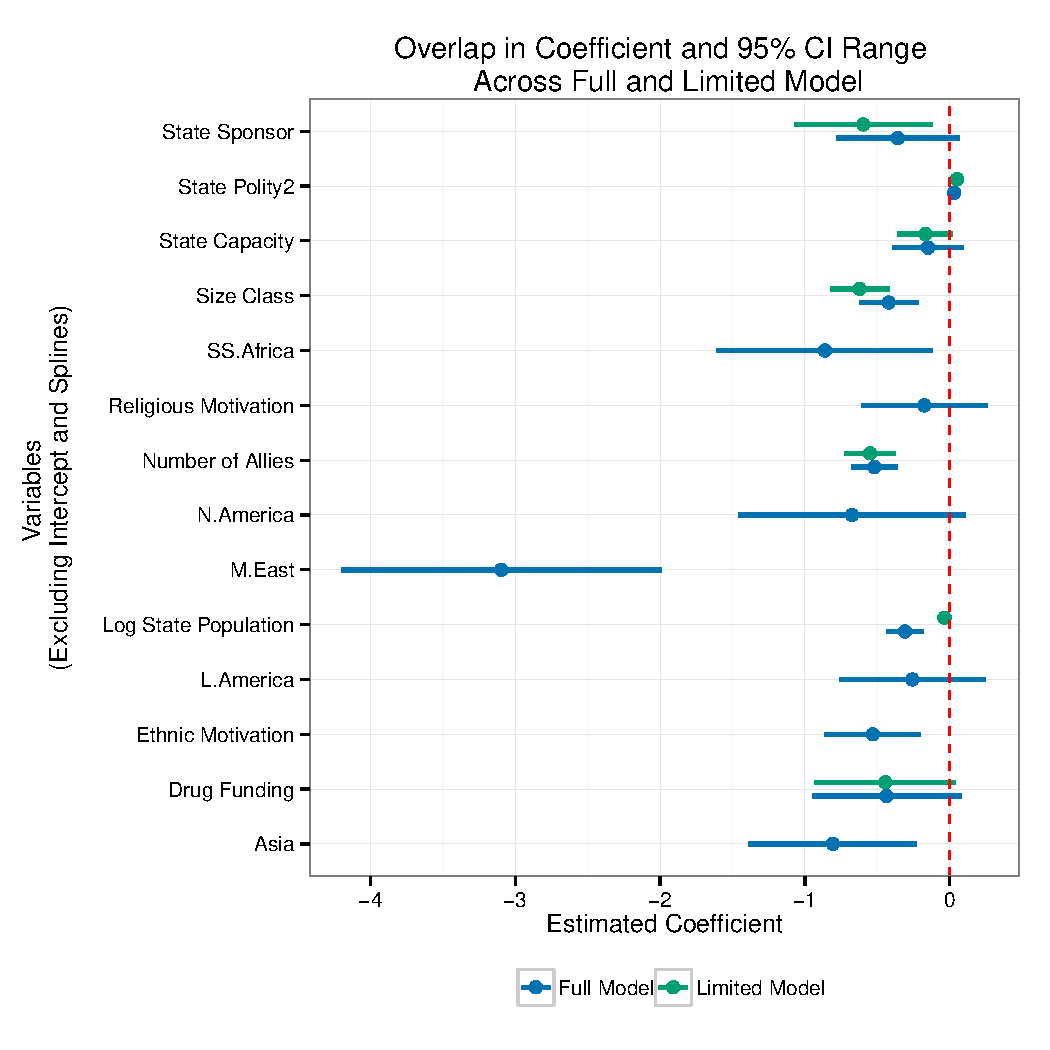
\includegraphics[width=78mm]{CoefPlotsBothModels.pdf}\\

\end{tabular}
\end{center}
\vspace{-17mm} 
\subsection*{Solution}
Estimating a parsimonious model with seven of the original independent
variables. The new model is consistent across six of the seven
IDVs, differing most on logged state population. Although the new model loses the impact of regional
dummies and religious motivation, the new model allows for inclusion of
community attributes.
}


%%%%%%%%%%%%%%%%%%%%%%%%%%%%%%%%%%%%%%%%%%%%%%%%%%%%%%%%%%%%%%%%%%%%%%%%%%%%%%
\headerbox{Extension: Extracting and Leveraging Network Information}
{name=networks,column=2,span=2}
{
The following two graphs replicate and extend the network graph that Phillips
used to generate his \textit{allies} and \textit{allies connections}
variables. I extended the network analysis to highlight densely
connected sub-graphs and to include both alliances and
rivalries. Network communities were
identified via a 5-step random walk procedure.
\vspace{-05mm}
\begin{center}
\begin{tabular}{ccc}
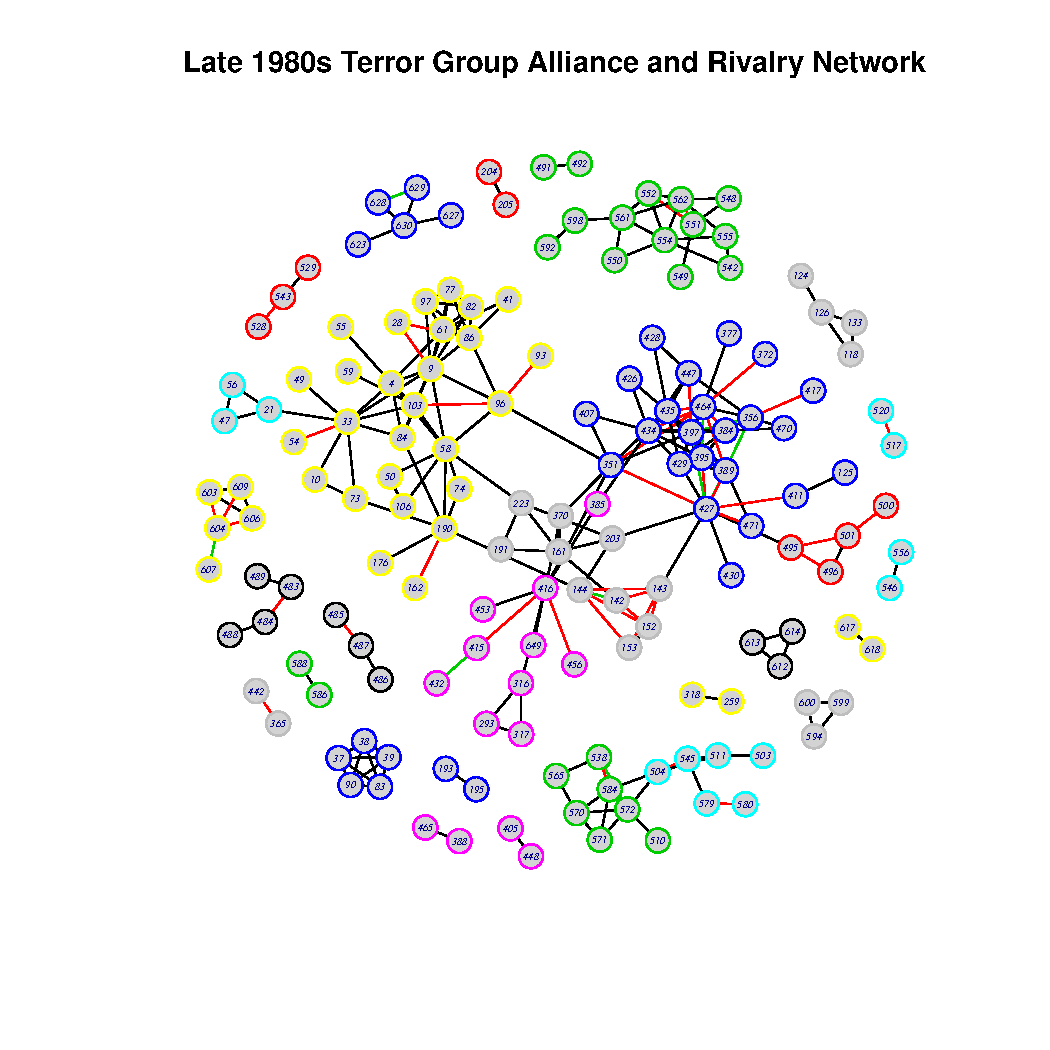
\includegraphics[height=92mm,width=81mm]{Poster_Final_80sNetwork.pdf}
  & 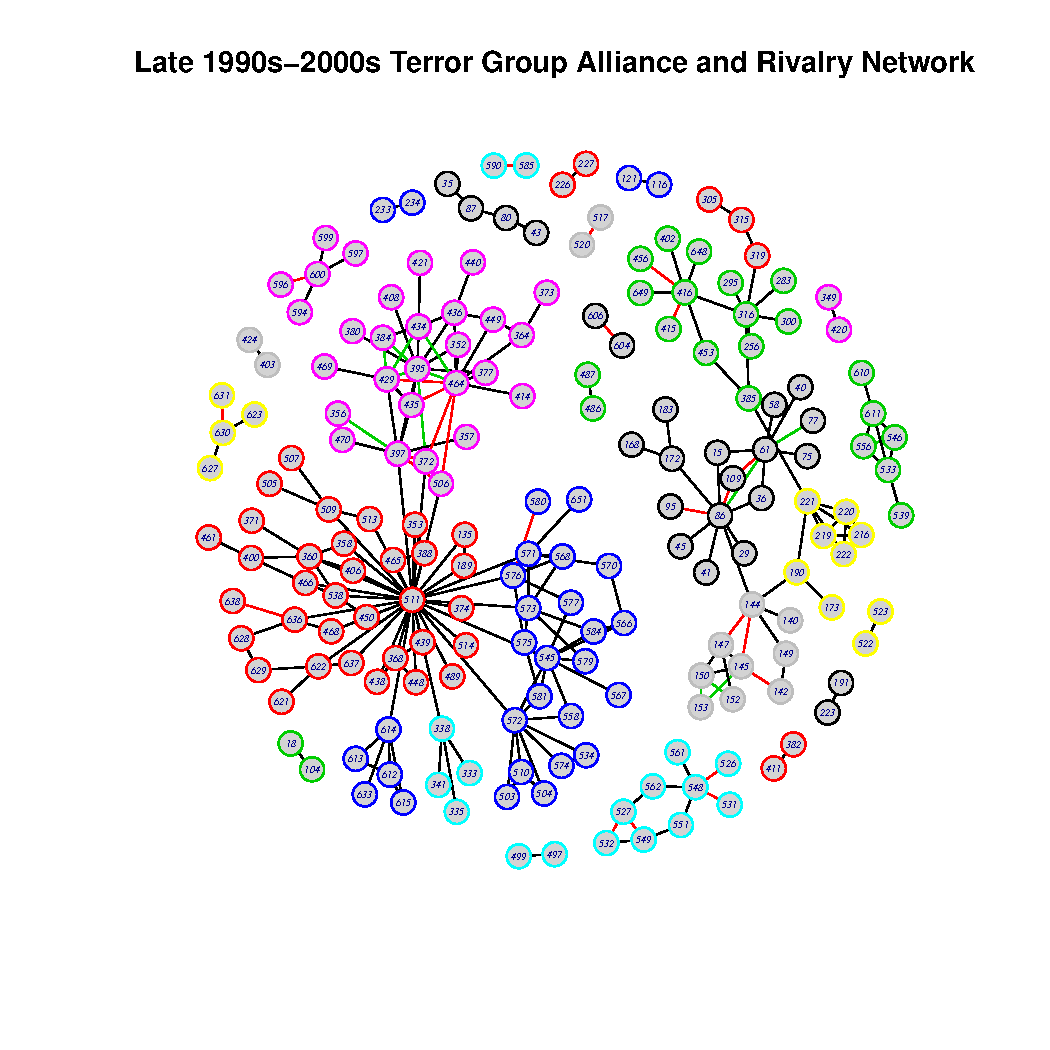
\includegraphics[height=92mm,width=81mm]{Paper_Graph_Nineties.pdf}\\
\end{tabular}
\end{center}
\vspace{-15mm}
Black edges show alliances, red edges show rivalries, and green edges
indicate that a dyad had experienced both alliances and rivalries.
Communities are indicated by the outline color of contiguous nodes.
}

%%%%%%%%%%%%%%%%%%%%%%%%%%%%%%%%%%%%%%%%%%%%%%%%%%%%%%%%%%%%%%%%%%%%%%%%%%%%%%

\headerbox{Extension: Quality or Quantity?}
{name=regsgraphs,column=2,below=networks, span=2}
{
The table on the left presents the results of estimating the modified
allies model with four large sub-communities included as binary
control variables. The right applies the modified model to four of the
largest sub-communities to investigate whether the estimates
change. Within these communities, the estimated coefficient for number of allies ceases to be statistically significant.
\vspace{-12mm}
\begin{center}
\begin{tabular}{cc}
 \\ [2.0ex]
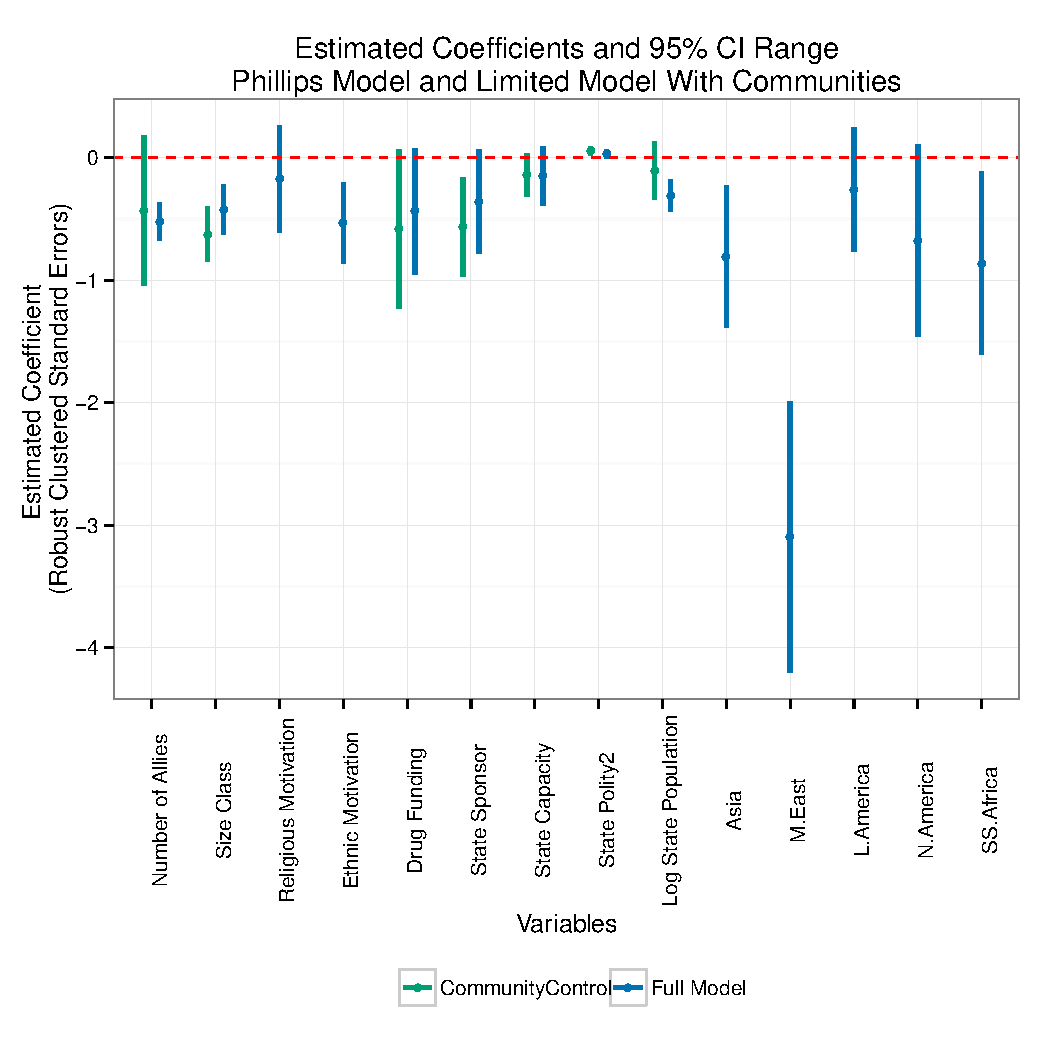
\includegraphics[height=65mm,width=70mm]{GeboandPaperTables.pdf}&
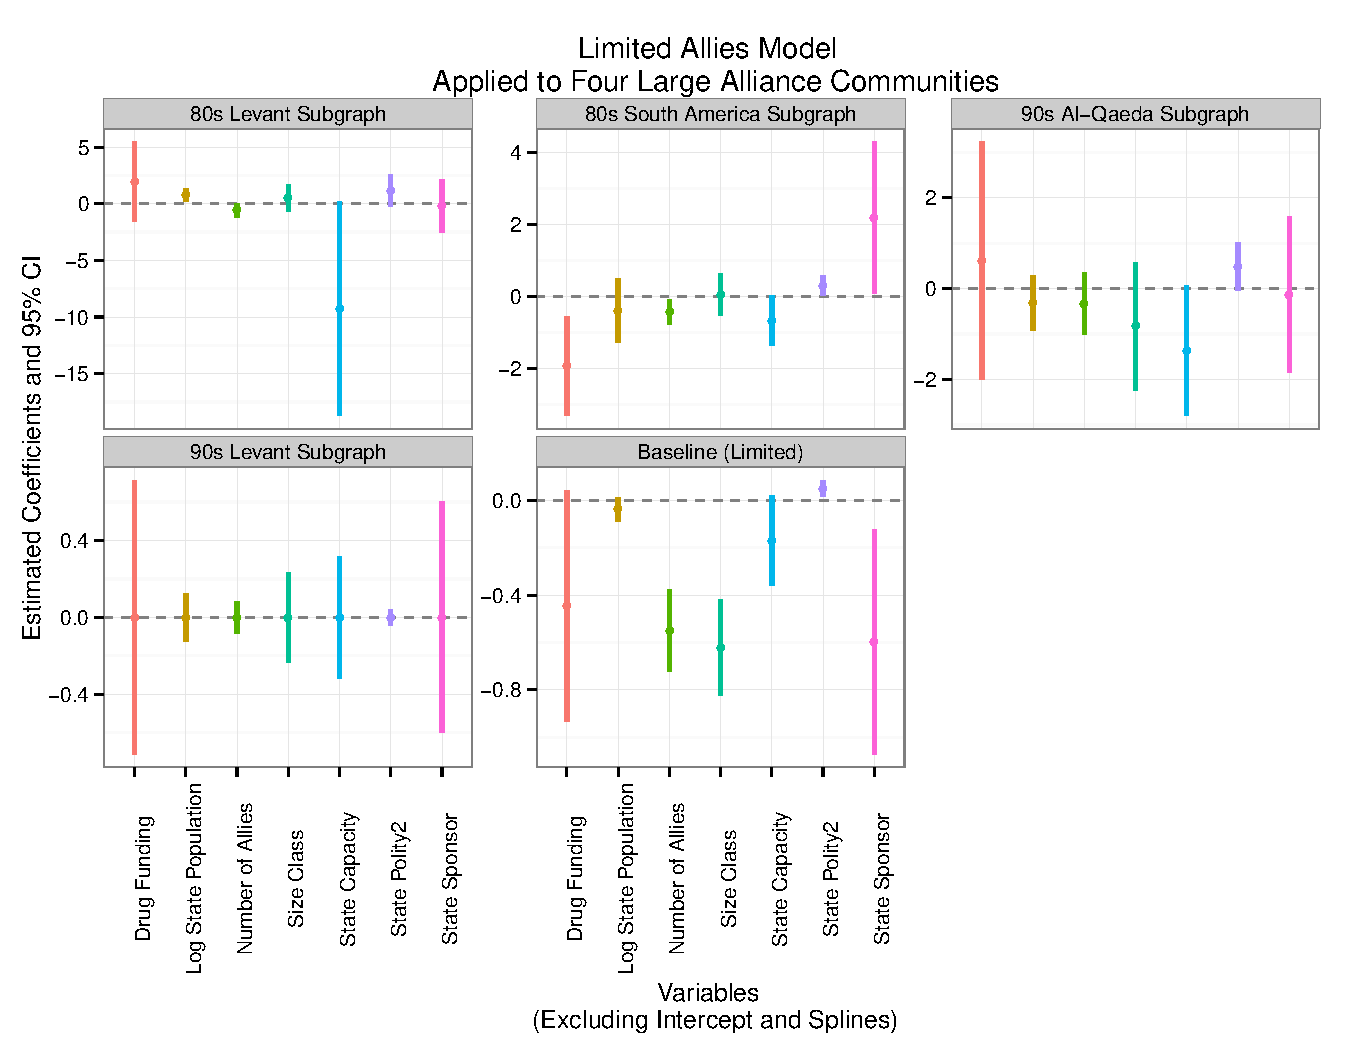
\includegraphics[height=65mm,width=90mm]{smallTableCoef.pdf}\\

\end{tabular}
\end{center}
\vspace{-4mm}
}


%%%%%%%%%%%%%%%%%%%%%%%%%%%%%%%%%%%%%%%%%%%%%%%%%%%%%%%%%%%%%%%%%%%%%%%%%%%%%%

\headerbox{Robustness of the Allies Model}
{name=xfold,column=1,span=1}
{
The coefficient plots indicate that the coefficient estimates of the
Allies model are generally robust out-of-sample tests on randomly
selected folds of the data. However, the ROC
plots show that predictive performance is sensitive
to which groups are included. AUC values for the out-of-sample data range from 0.72 to 0.873, with an
average of .804.

\vspace{-1mm}
\begin{center}
\begin{tabular}{c}
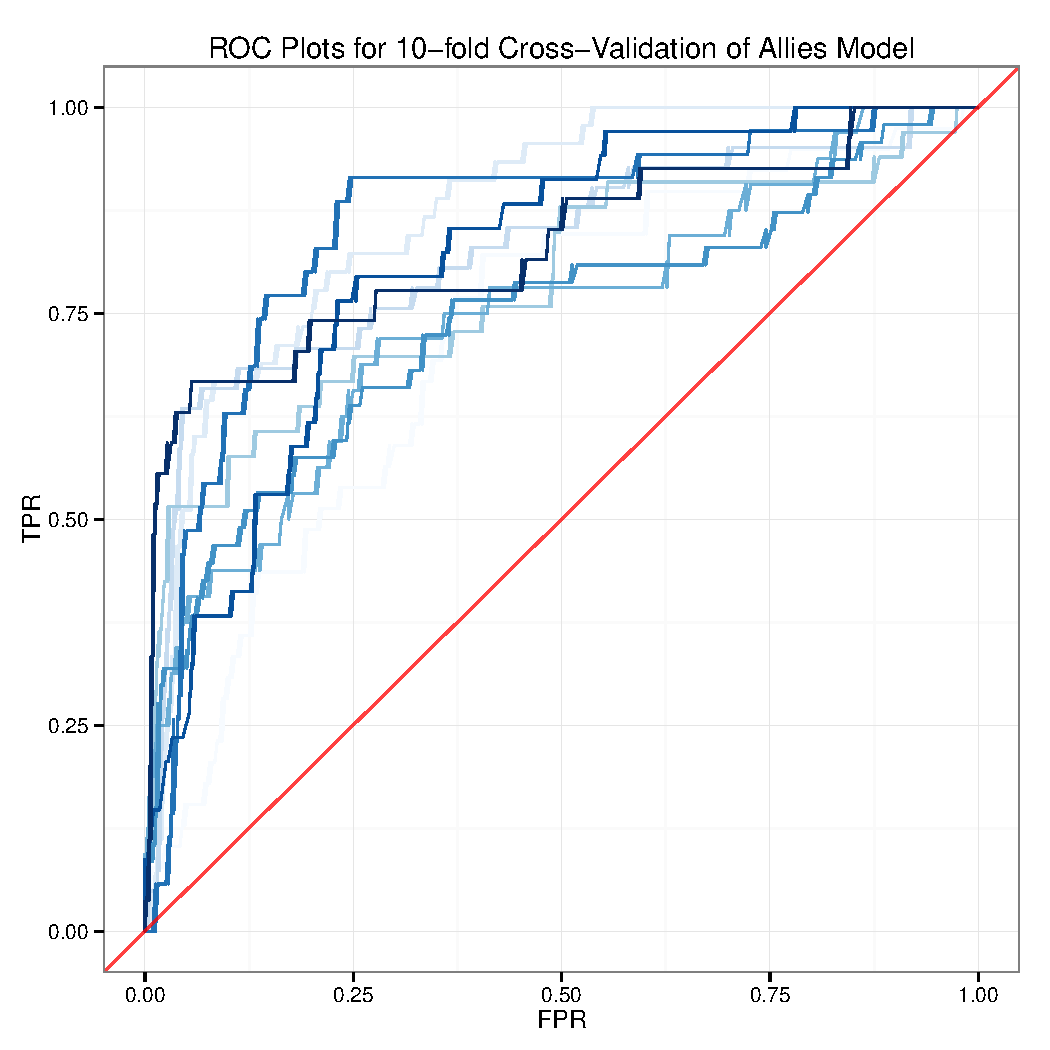
\includegraphics[height=45mm,width=60mm]{XfoldRocplot.pdf}\\
 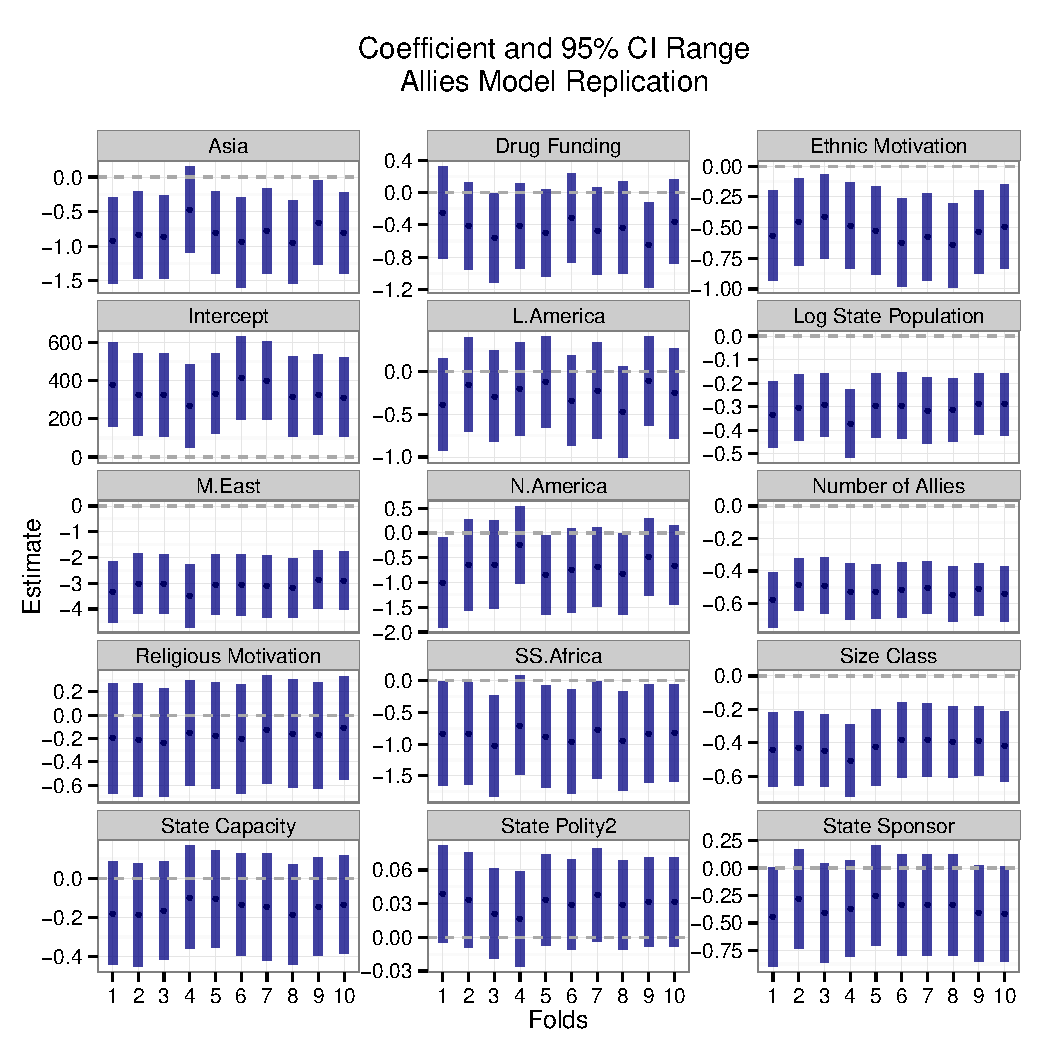
\includegraphics[height=45mm,width=60mm]{XVal_Poster_coefPlots.pdf}\\
\vspace{-10mm}
\end{tabular}
\end{center}
\vspace{3mm}

}

%%%%%%%%%%%%%%%%%%%%%%%%%%%%%%%%%%%%%%%%%%%%%%%%%%%%%%%%%%%%%%%%%%%%%%%%%%%%%%

\headerbox{Predictive Power of the Allies Model}
{name=sepplots,column=1,span=1, below=xfold}
{
The Allies model suffers from consistently high false negative predictions both in the full model (large plot) and in the training sets of the
cross-validation (small plots). This characteristic potentially reflects the
strategic interplay between groups and security organizations or
signals an underlying duration-enhancing attribute omitted from the Allies model.
\vspace{-05mm}
\begin{center}
\begin{tabular}{c}
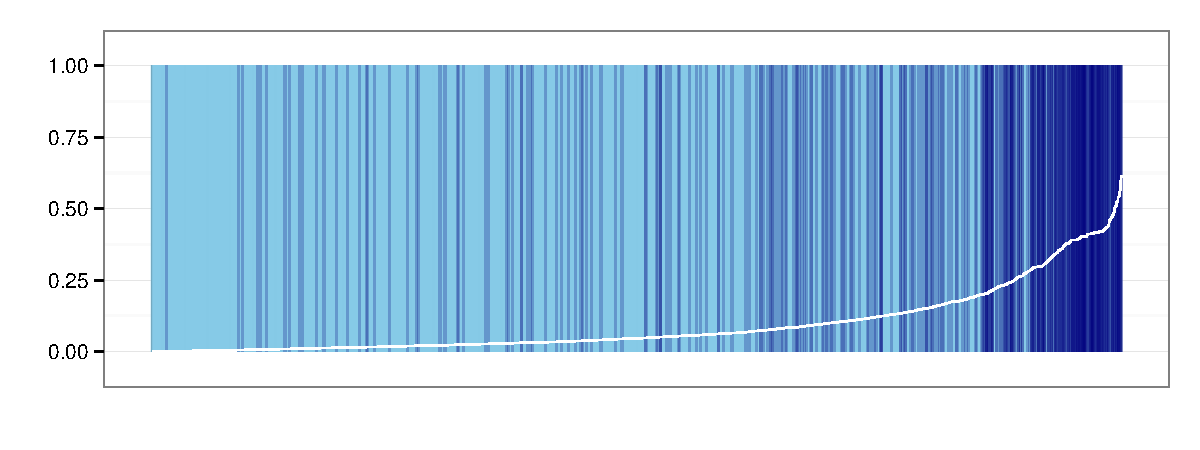
\includegraphics[height=27mm,width=81mm]{separationplotfullmodelSepPlot.pdf}\\
\vspace{-08mm}
\end{tabular}
\begin{tabular}{lcr}
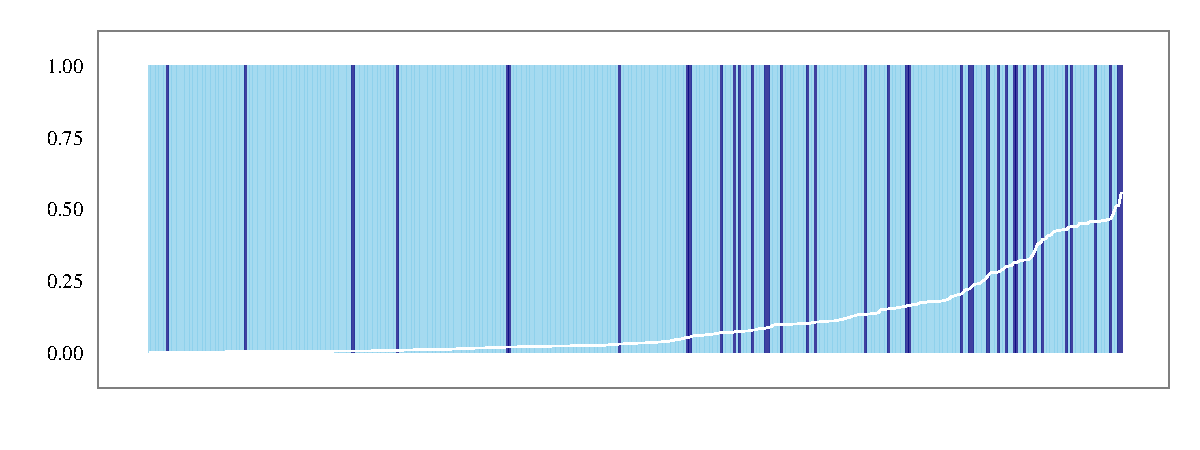
\includegraphics[height=9mm,width=36mm]{separationplotsepDat1.pdf}& & 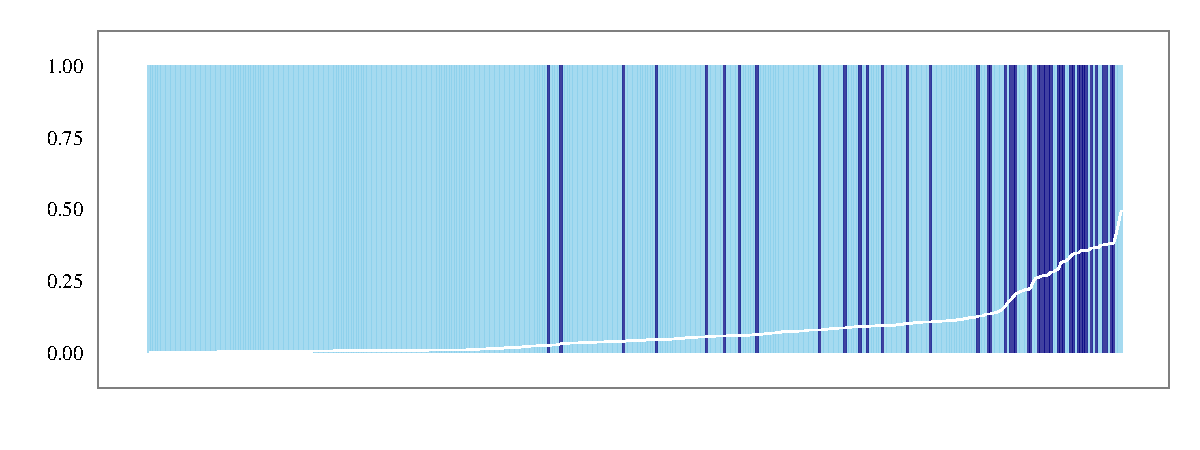
\includegraphics[height=9mm,width=36mm]{separationplotsepDat2.pdf}\\
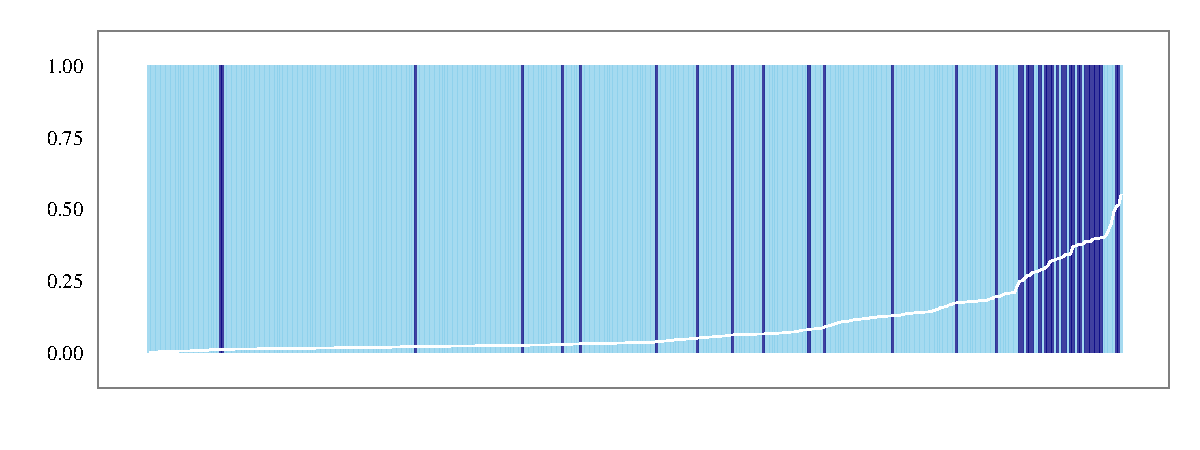
\includegraphics[height=9mm,width=36mm]{separationplotsepDat3.pdf}& & 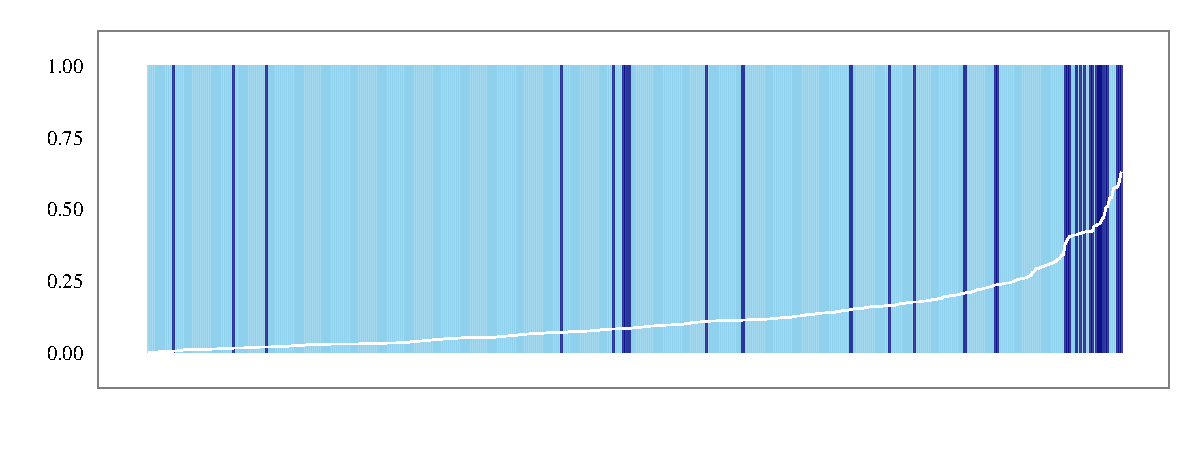
\includegraphics[height=9mm,width=36mm]{separationplotsepDat4.pdf}\\
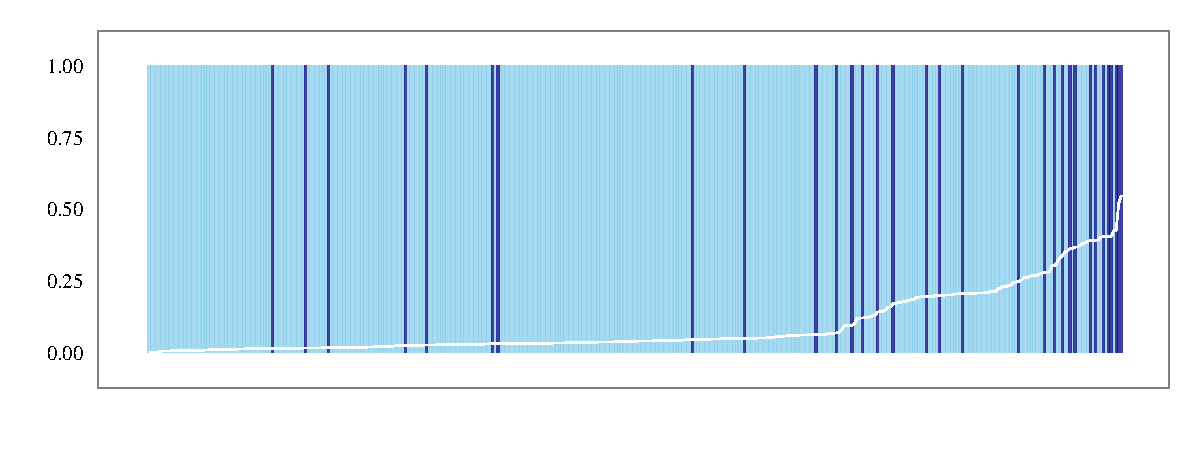
\includegraphics[height=9mm,width=36mm]{separationplotsepDat5.pdf}& & 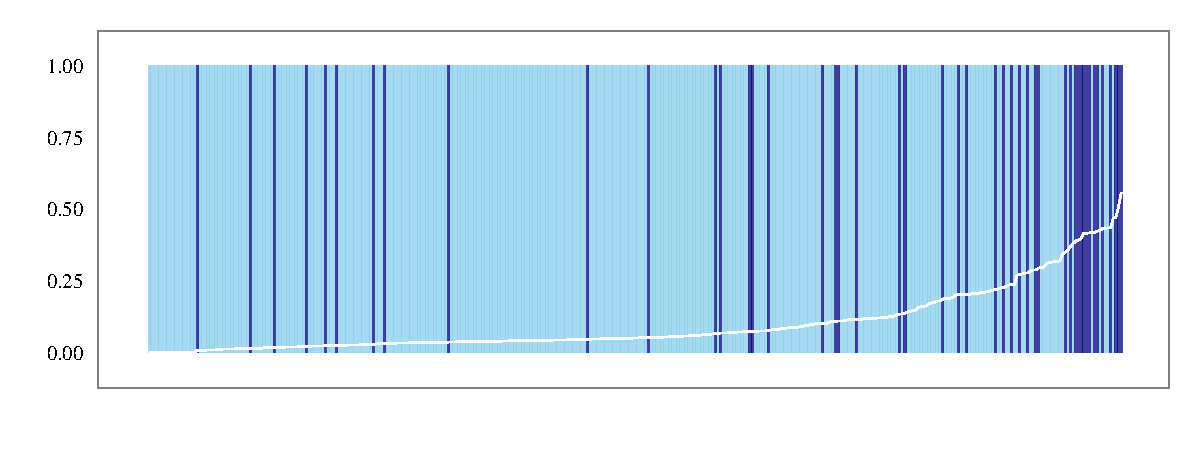
\includegraphics[height=9mm,width=36mm]{separationplotsepDat6.pdf}\\
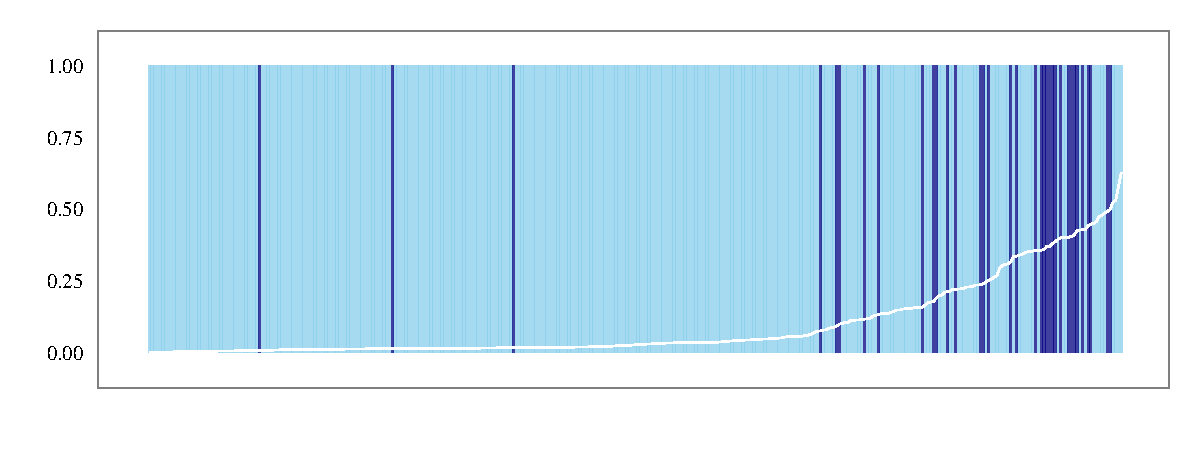
\includegraphics[height=9mm,width=36mm]{separationplotsepDat7.pdf}& & 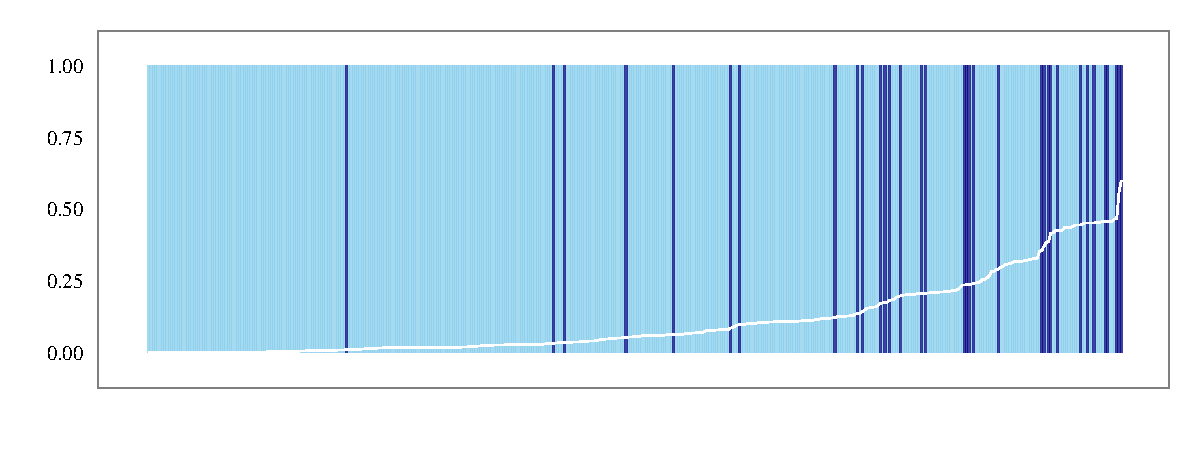
\includegraphics[height=9mm,width=36mm]{separationplotsepDat8.pdf}\\
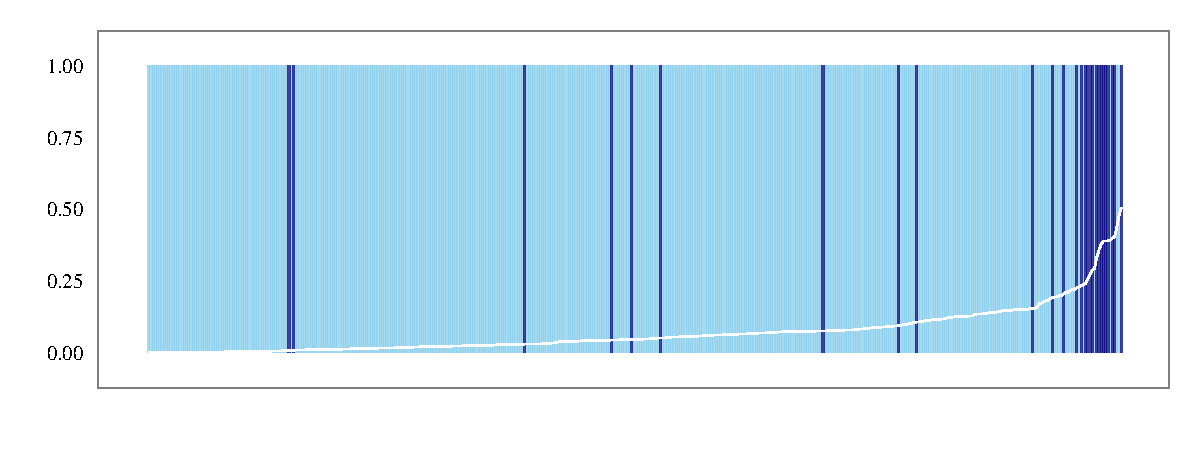
\includegraphics[height=9mm,width=36mm]{separationplotsepDat9.pdf}& & 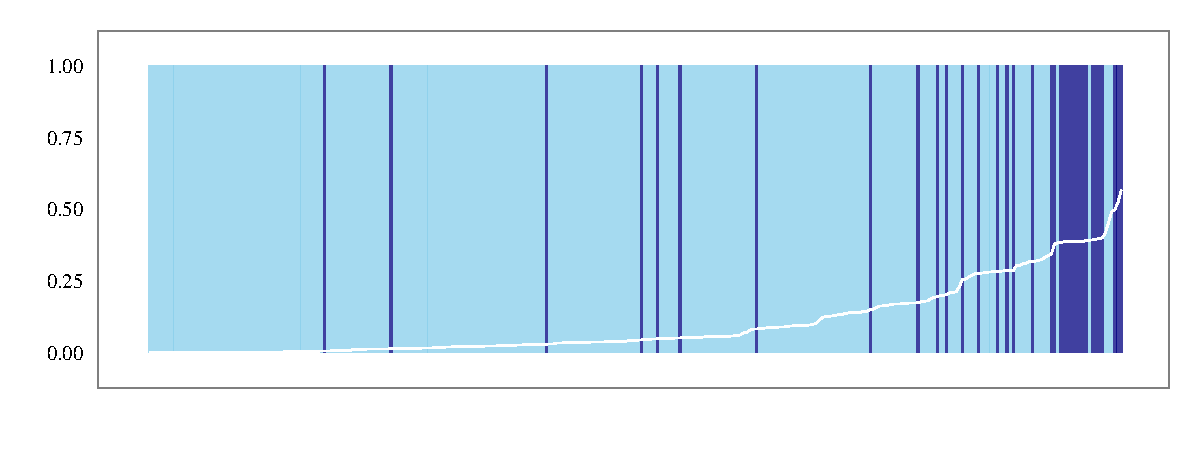
\includegraphics[height=9mm,width=36mm]{separationplotsepDat10.pdf}\\
\vspace{-6mm}
\end{tabular}
\end{center}
}


%%%%%%%%%%%%%%%%%%%%%%%%%%%%%%%%%%%%%%%%%%%%%%%%%%%%%%%%%%%%%%%%%%%%%%%%%%%%%%

\headerbox{Marginal Effects of Allies in Base Model}
{name=margeffects,column=0,span=1, below=data}
{

The four panels below show the changes in predicted probability of failure
as number of allies increases, estimated at the beginning and end of
each data collection wave. Notably, the effect diminishes with time.
\vspace{-2mm}
\begin{center}
\begin{tabular}{c}
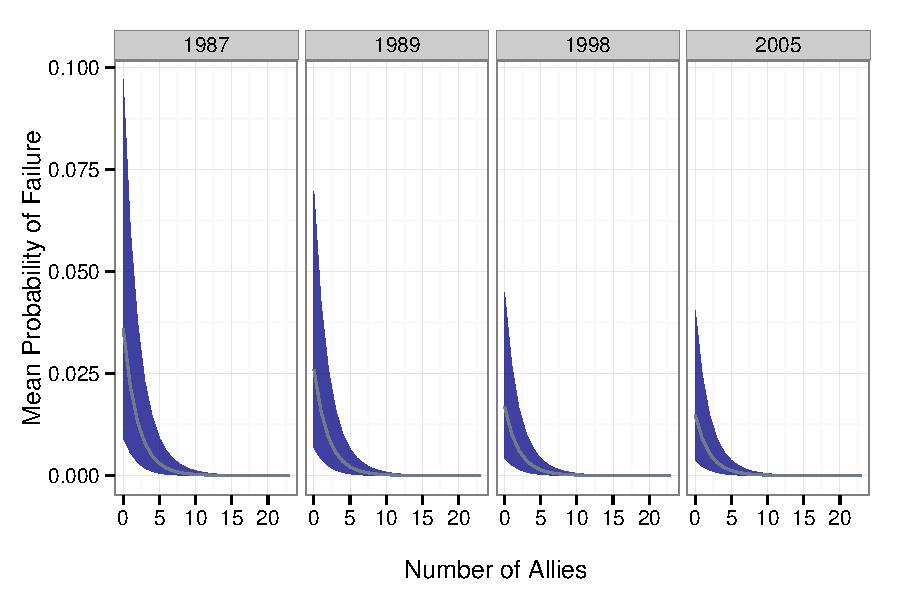
\includegraphics[height=32mm, width=59mm]{AlliesSimulations.pdf}\\
\vspace{-5.5mm}
\end{tabular}
\end{center}
}

%%%%%%%%%%%%%%%%%%%%%%%%%%%%%%%%%%%%%%%%%%%%%%%%%%%%%%%%%%%%%%%%%%%%%%%%%%%%%%
\headerbox{Conclusions}
{name=conclusion,column=2,row=2,span=1,below=regsgraphs}
{
\begin{itemize}
\item Controlling for large communities removes
  statistical significance of number of allies variable.  This
  suggests that the overall number of allies is less important than
  the quality of those allies. 
\item Unexpectedly, controlling for large communities makes
  having a state sponsorship significantly associated with duration.
\end{itemize}
\vspace{-4.0mm}
}


%%%%%%%%%%%%%%%%%%%%%%%%%%%%%%%%%%%%%%%%%%%%%%%%%%%%%%%%%%%%%%%%%%%%%%%%%%%%%%
\headerbox{Future Avenues}
{name=conclusion,column=3,row=2,span=1,below=regsgraphs}
{

\begin{itemize}
\item Address missing Polity2 data for Afghanistan, Cambodia, Iraq,
  Lebanon, and Surname. 
\item Expand model using a multi-level approach to allow for possible
  community-specific effects.
\item Explore robustness and predictive power of community extension.
\end{itemize}
}




\end{poster}
\end{document}